% =============================================================
%  SUPPLEMENTARY MATERIAL
%  Body content for the standalone supplementary document
%  (compiled via supplementary_main.tex).
% =============================================================
\setcounter{figure}{0}
\renewcommand{\thefigure}{S\arabic{figure}}
\setcounter{section}{0}
\renewcommand{\thesection}{S\arabic{section}}

\section*{Supplementary Data}

% ----- Figure S1 -----
\begin{figure}[ht]
\centering
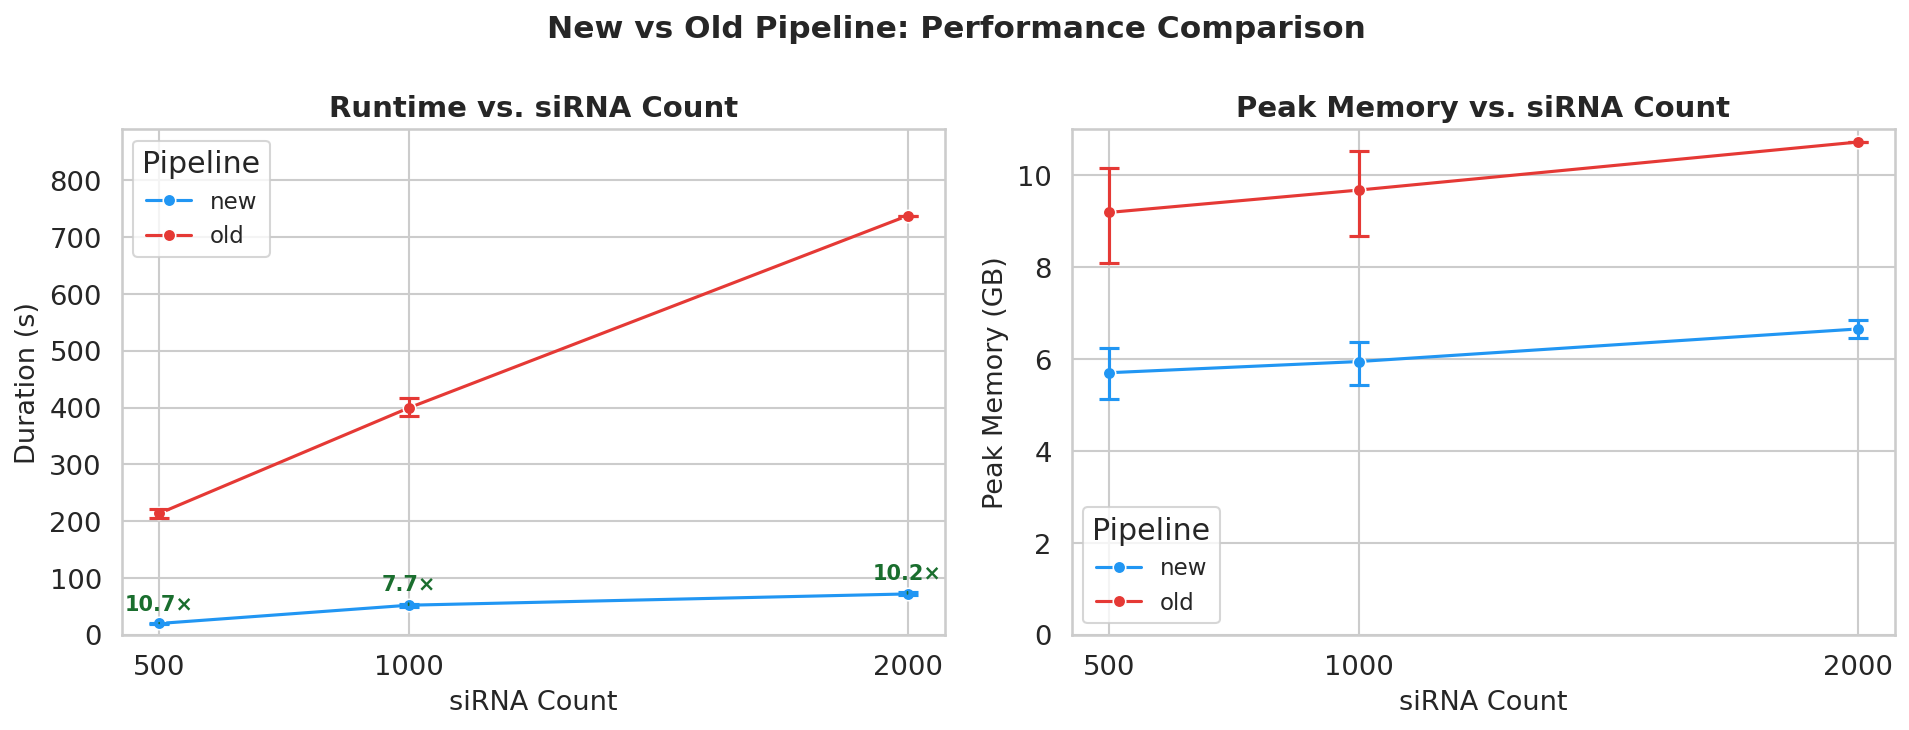
\includegraphics[width=\linewidth]{figures/pipeline_comparison}
\caption{%
  \textbf{Wall-clock time and peak memory of RIOT versus the legacy pipeline
  across batch sizes.}
  Each box spans the interquartile range of five independent randomised trials;
  the central line marks the median; whiskers extend to the full range.
  \textbf{(A)}~Wall-clock time (seconds) for the intersection, accessibility
  annotation, Boltzmann partition-function, and output stages on 500, 1{,}000,
  and 2{,}000 siRNAs from the Hüsken et~al.\ genome-wide efficacy
  library~\citep{huesken2005design}.
  RIOT achieves a $7.7{-}10.7\times$ speed-up relative to the legacy
  Python~2.7 implementation.
  \textbf{(B)}~Peak resident-set size (GB) of the parent process as reported
  by \texttt{/usr/bin/time -v}.
  RIOT plateaus at $\approx$7\,GB regardless of batch size;
  the legacy pipeline grows from $\sim$8.5\,GB to $\sim$10\,GB as batch
  size increases.
  Benchmarks were run on an AMD EPYC 9554 server (64 physical cores)
  with 32 workers for both pipelines; pre-computed RIsearch2 binding-site
  predictions were provided as input so that search time is excluded from
  both measurements (see Supplementary Methods).%
}
\label{fig:S1}
\end{figure}

% =============================================================
%  SUPPLEMENTARY METHODS
% =============================================================
\section*{Supplementary Methods}

\subsection*{RIOT pipeline stages and partition-function model}

The four-stage model of \citet{alkan2017risearch2} is preserved.
In the first stage, siRNA--target interaction predictions
are generated by calling \texttt{risearch.index()} to build the suffix-array
index of the target and \texttt{risearch.search()} to locate binding sites, both
invoked directly through the Python bindings, returning results as a Polars
DataFrame in the same process with no intermediate files on disk.
In the second stage, predicted binding sites are intersected with an expression
annotation (GTF or BED) to retain sites overlapping expressed features and to
assign position-specific abundance values. Intersection is performed in-memory
using an NCLS interval index~\citep{ncls} partitioned by chromosome and strand,
with chromosome--strand pairs distributed across a thread pool; no external tools
such as \texttt{bedtools} are needed.
In the third stage, per-site binding-site opening energies $O_i = -RT\ln p_i$
are either computed on-the-fly from a genome FASTA or read from per-chromosome
Parquet profiles pre-computed by the \texttt{accessibility} subcommand, in both
cases using the RNAplfold algorithm (ViennaRNA~2.7.2 Python
API~\citep{lorenz2011vienna}; $W{=}80$, $L{=}40$, $u{=}30$) at the same
temperature used for the partition function, so that $E^\prime_i$ and $O_i$ are
on a consistent thermodynamic scale. The Boltzmann-weighted sum
%
\begin{equation}
  Z_s = \sum_{i \in \mathcal{I}_s}
        A_i \,
        \exp\!\left(\frac{-\bigl(E^\prime_i + O_i\bigr)}{RT}\right)
  \label{eq:partition}
\end{equation}
%
\noindent is evaluated as a single vectorised \texttt{group\_by} aggregation
in Polars, where $A_i$ is the transcript expression level,
$E^\prime_i$ is the RIsearch hybridisation energy,
$O_i = -RT\ln p_i$ is the opening energy derived from the RNAplfold unpaired
probability $p_i$, $R = 1.987\times10^{-3}$\,kcal\,mol$^{-1}$\,K$^{-1}$ is
the molar gas constant, and $T$ is the folding temperature (default
$310.15$\,K, $37\,^\circ$C). When an on-target binding site is supplied via
\texttt{-{}-on-target-ids}, its Boltzmann weight $W_{\mathrm{on}}$ is computed
identically and added to $Z_s$; the on-target probability
$p_{\mathrm{on}} = W_{\mathrm{on}} / Z_s$ determines the aggregate
off-targeting potential $P_{\mathrm{OFF}} = 1 - p_{\mathrm{on}}$.
Per-transcript off-targeting probabilities $p_{\mathrm{off},i} = W_i / Z_s$ are
then computed as column operations on the resulting DataFrame. Parametric sweeps
over $\alpha$, $\gamma$, and $\theta$ are resolved in a single aggregation pass
rather than repeated sequential iterations. In the fourth stage, results are
written incrementally as each siRNA completes, in TSV, CSV, or Parquet format.

\subsection*{Parallelism and memory}

When processing a directory of per-siRNA prediction files, RIOT
distributes work across a configurable process pool. A spawn-based
multiprocessing context is used to avoid interaction with the Rayon thread
pool used internally by Polars. The expression annotation is loaded once
into Arrow IPC format and memory-mapped into each worker process via the
operating-system page cache, keeping peak memory proportional to a single
annotation copy regardless of worker count. Each worker performs the
intersection, accessibility lookup, and partition-function evaluation for one
siRNA at a time; prediction files are parsed lazily so that only filtered,
selected columns are materialised, and output is streamed to disk incrementally
throughout a batch run.

\subsection*{Benchmark dataset}

The benchmark uses a subset of the genome-wide siRNA efficacy library of
\citet{huesken2005design}, which comprises 2{,}431 chemically synthesised
21-mer siRNAs targeting 34 human genes, with experimentally measured
knockdown efficacies obtained in the H1299 non-small-cell lung carcinoma
cell line.
A master set of 2{,}000 siRNAs was drawn by uniform random sampling (without
replacement) from this library; smaller batch sizes of 1{,}000 and 500 were
produced by further subsampling from this master set, with a fresh random
draw for each of the five independent benchmark iterations.
Target sequences for the off-target search were derived from the
GRCh38/hg38 reference genome (UCSC assembly, December 2013).
Expression values were taken from an H1299 RNA-seq experiment
(ArrayExpress accession E-MTAB-2770), converted to per-transcript
read counts and stored in BED format.

\subsection*{Genome indexing and RIsearch2 binding-site search}

The hg38 reference genome was indexed with RIsearch2 to
produce a suffix-array package file (\texttt{hg38.pksuf}):

\begin{verbatim}
risearch2.x -c hg38.fa -o hg38.pksuf
\end{verbatim}

\noindent where \texttt{-c} specifies the target FASTA to index and
\texttt{-o} names the output suffix-array package.
Binding-site predictions for each siRNA were generated once and stored
as compressed output files; this search step was excluded from all
pipeline benchmark timings so that only the post-search processing
stages (intersection, accessibility annotation, partition function, and
output) are measured.

The search command used was:

\begin{verbatim}
risearch2.x \
    -i hg38.pksuf \
    -q huesken_sirnas.fa \
    -s 2:7 \
    -e -10 \
    -p2 \
    -l 25 \
    -t 32
\end{verbatim}

\noindent Key flag meanings:
\begin{itemize}
  \item \texttt{-i hg38.pksuf} — pre-built suffix-array index of the
    hg38 target.
  \item \texttt{-q huesken\_on\_subset.fa} — FASTA file of siRNA query
    sequences (guide strand, 5$'$$\to$3$'$).
  \item \texttt{-s 2:7} — restrict seed matches to guide-strand positions
    2–7 (the canonical seed region for RISC-mediated target recognition).
  \item \texttt{-e -10} — energy threshold of $-10$\,kcal\,mol$^{-1}$;
    candidate sites with a hybridisation energy above this value are
    discarded.
  \item \texttt{-p2} — bindingsite output format, reporting one line per
    predicted interaction with genomic coordinates, energies, and alignment.
  \item \texttt{-l 25} — minimum alignment length of 25\,nt, filtering
    out truncated partial matches at sequence boundaries.
  \item \texttt{-t 32} — use 32 parallel threads for the search.
  \item \texttt{--verbose} — write progress information to standard error.
\end{itemize}

\subsection*{H1299 expression annotation}

Per-transcript expression weights for the H1299 (NCI-H1299, large-cell lung
carcinoma) cell line were derived from the RNA-seq dataset E-MTAB-2770
(\textit{RNA-Seq of 675 human cancer cell lines}, CCLE), which is archived at
ArrayExpress and contains data for approximately 675 cancer cell lines.

\paragraph{Sample identification.}
The SDRF file was queried to identify the single H1299 paired-end run,
yielding accession \texttt{SRR8615898}
(R1: 4.7\,GB; R2: 4.8\,GB).

\paragraph{Reference genome and annotation.}
GENCODE~v47 was used as the reference (GRCh38 coordinate space):
\texttt{gencode.v47.transcripts.fa.gz} for Salmon index construction and
\texttt{gencode.v47.annotation.gtf.gz} for transcript coordinates.

\paragraph{Quantification.}
A Salmon~v1.10.3 quasi-mapping index was built from the GENCODE transcript
sequences with the \texttt{-{}-gencode} flag (strips pipe-delimited header
fields so transcript IDs match the GTF).
Paired-end reads were quantified with:

\begin{verbatim}
salmon quant \
    -i input/salmon_index \
    -l A \
    -1 SRR8615898_1.fastq.gz \
    -2 SRR8615898_2.fastq.gz \
    -p 16 \
    --validateMappings \
    --gcBias \
    -o input/quant/SRR8615898
\end{verbatim}

\noindent Key flags: \texttt{-l~A} auto-detects library strandedness;
\texttt{-{}-validateMappings} applies alignment scoring to filter spurious
mappings; \texttt{-{}-gcBias} corrects for GC-content bias.
The run achieved an 87.6\% mapping rate.

\paragraph{BED7 construction.}
Salmon output (\texttt{quant.sf}, 384{,}354 transcript rows) was merged with
GTF transcript-level coordinates using a custom script (\texttt{make\_bed7.py}).
Each GTF \texttt{transcript} record was converted to 0-based BED coordinates
(BED start $=$ GTF start $- 1$; end unchanged) and joined to its TPM value
by versioned ENST identifier.
Transcripts absent from the Salmon output (PAR-locus duplicates and assembly
patches) received TPM $= 0$.
The output file (\texttt{annotation\_E-MTAB-2770\_GRCh38\_v47.bed}) is a
tab-separated BED7 file (385{,}659 rows; no header) in which column~7 carries
the per-transcript TPM as a floating-point value:

\begin{center}
\small
\begin{tabular}{lllllll}
\hline
chrom & start & end & transcript\_id & . & strand & TPM \\
\hline
chr12 & 6534516 & 6538371 & ENST00000229239.10 & . & + & 6130.06 \\
\hline
\end{tabular}
\end{center}

Of the 385{,}659 transcripts, 143{,}881 (37.3\%) carried TPM $> 0$,
consistent with the fraction of GENCODE transcripts detectably expressed in
a single cell-line condition.
Transcripts with TPM $= 0$ are retained in the file because the intersection
service reads the annotation as a single indexed structure; dropping unexpressed
entries would misalign row offsets.
The high GAPDH TPM (ENST00000229239.10: 6{,}130) confirms biologically
plausible quantification.

\subsection*{Benchmark protocol}

Timing and peak-memory measurements were collected on a server equipped
with an AMD EPYC~9554 processor (64 physical cores, 128 threads) and
sufficient RAM to keep all input files resident.
Both pipelines used 32 parallel workers (\texttt{-j~32} for GNU parallel
in the legacy case; \texttt{-j~32} process-pool workers for the new
pipeline).

For each combination of pipeline version (new / legacy) and batch size
(500, 1{,}000, 2{,}000 siRNAs), the following procedure was applied:
(i)~one warmup run was executed and discarded to populate OS page-cache
entries and JIT any Python bytecode; (ii)~five timed runs were executed,
each with a fresh output directory to avoid I/O caching effects.
Wall-clock time and peak resident-set size (RSS) of the parent process
were recorded with \texttt{/usr/bin/time -v} (GNU~time).
Because both pipelines spawn independent child processes (GNU~parallel in
the legacy case; a spawn-based process pool in RIOT), the RSS
reported reflects only the parent; aggregate memory across all 32 workers
will exceed this figure.

For batch sizes of 1{,}000 and 500, each of the five timed runs used an
independently drawn random subset of the master 2{,}000-siRNA set,
ensuring that variance estimates reflect genuine sampling variability
rather than run-to-run measurement noise alone.
Pre-computed RIsearch2 binding-site prediction files were provided as
input to both pipelines, so that search time is excluded from all
measurements.

\subsection*{Accessibility pre-computation}

The legacy pipeline computed per-nucleotide RNA opening energies with a
Python~2.7 script that wrapped the \texttt{RNAplfold} executable
(ViennaRNA~2.6.3) as a subprocess, emitting two flat \texttt{uint8} binary
files per chromosome (one per strand). RIOT's \texttt{accessibility}
subcommand reproduces the same folding parameters ($W{=}80$, $L{=}40$,
$u{=}30$) through the ViennaRNA~2.7.2 Python API directly, without spawning
subprocesses: for each chromosome the call
\texttt{RNA.fold\_compound(...).probs\_window(...)} returns per-position
unpaired-probability vectors at the specified temperature (default
37\,$^\circ$C, set via \texttt{-{}-temperature}), from which opening energies
$O_i = -RT\ln p_i$ are computed in-process and written as a single
per-chromosome Apache Parquet file with columnar compression and zero-copy
Arrow reads.

\paragraph{Accessibility pre-computation benchmark.}
Folding the complete GRCh38/hg38 reference ($W{=}80$, $L{=}40$, $u{=}30$,
64 workers on the AMD EPYC~9554 server) was compared between the legacy script
(driven by GNU~\texttt{parallel}) and RIOT's \texttt{accessibility} subcommand
(Table~\ref{tab:acc-bench}). RIOT completes the full-genome
fold $\sim$34\% faster (8\,h\,45\,m vs.\ 13\,h\,12\,m) and stores the resulting
profiles in $\sim$42\% less disk space (105\,GB vs.\ 180\,GB), the latter
because each chromosome is written as a single two-strand compressed Parquet
file rather than two uncompressed binary files. The trade-off is higher peak
resident memory ($\sim$3.6\,GB vs.\ $\sim$309\,MB, roughly $12\times$), as the
ViennaRNA Python API holds per-chromosome probability matrices in memory rather
than streaming them through a subprocess; both figures are small relative to
typical server memory, and this cost is incurred only once per genome and
folding condition.

\begin{table}[ht]
\centering
\caption{Full-genome accessibility pre-computation: legacy script versus
RIOT's \texttt{accessibility} subcommand (hg38; $W{=}80$, $L{=}40$, $u{=}30$;
64 workers).}
\label{tab:acc-bench}
\small
\begin{tabular}{lrr}
\hline
Metric & Legacy & New \\
\hline
Wall-clock time      & 13\,h\,12\,m & 8\,h\,45\,m \\
Peak resident memory & $\sim$309\,MB & $\sim$3.6\,GB \\
On-disk profile size & 180\,GB      & 105\,GB \\
Files per chromosome & 2            & 1 \\
\hline
\end{tabular}
\end{table}
\section{Temperature dependent energy parameters}\label{temperature-dependent-energy-parameters}
Notation, N indicates an unknown nucleotide. In the stacking energies, the N is
substituted with a nucleotide (ACGT/U) giving the stack the highest possible
energy. \_ indicates gap, a missing nucleotide, at the corresponding position,
that is a bulge on the strand opposite the gap.
\begin{verbatim}
RNA: rA,rC,rG,rU,rN,r\_
DNA: dA,dC,dG,dT,dN,d\_

RNA/RNA: 5'-AC-3' bound to 3'-UG-5': rACUG
DNA/DNA: 5'-AC-3' bound to 3'-TG-5': dACTG
RNA/DNA: 5'-rAC-3' bound to 3'-dTG-5': rACdUG
\end{verbatim}

The energy model of RIsearch is the sum of the energies of nucleotide stacks,
where a stack is two nucleotides bound (aligned) to two nucleotides on the
opposite strand or aligned to gaps on the opposite strand when the alignment
contains bulges / gaps. A particular case is the stacks initiating or
terminating the binding, which are written as, e.g. \_G\_C and G\_C\_,
respectively. These stacks are not allowed in other places in the alignment.

The binding energy matrices are derived from those in ViennaRNA\cite{ref4},
which are again derived from the nearest neighbor energy model parameters from
papers\cite{ref5,ref6,ref7,ref8,ref9,ref10,ref11,ref12} cited by ViennaRNA.
\begin{verbatim}
RNA/RNA: 2.6.3 RNAduplex

DNA/DNA: 2.6.3 RNAduplex -P DNA

RNA/DNA: 2.1.9h RNAduplex (in source code and binary only)
\end{verbatim}

The RNA/RNA and DNA/DNA matrices are implemented in all later versions of
ViennaRNA. However, the RNA/DNA matrices are only found in version 2.1.9h,
where they are the default in certain programs including RNAduplex. The first
(target) sequence must be the RNA, and the second the DNA, and these should be
entered with the corresponding alphabets, that is with U or T, respectively.

When we allow GAPS along with the standard nucleotides, we have $5^4 = 625$ stacking energy parameters (SEP) we need to obtain values for in each of the four cases. However, not all SEPs are allowed, e.g. an alignment must start and end with a binding pair (\_G\_C is defined, but not \_G\_A) and a gap on both strands is not allowed. In addition, some SEPs are identical due to the nature of the underlying chemistry (rGCAU is the same as rUACG, but rGCdAT is not the same as rUAdCG) and some SEPs are linearly dependent due to the nature of the model (a gap opened must also be closed (an example gap opening could be rAAU\_ and a closing could be rAA\_U).

The undefined SEPs are set to a large positive energy (+20.0 kcal/mol) in the energy matrices, and we enforce linear dependencies according to the rules below

\begin{enumerate}
\item A stack of nucleotides is, e.g. rACGU or rACdGT is written as $(\mathit{ijkl})$

\item Nucleotide are considered pairing when one of AU, AT, CG, GU and GT

\item If $i$ is paired but $j$ is not paired: $(\mathit{ijkl}) = (\mathit{jilk})$, e.g. rACdGG = rCAdGG

\item For RNA/RNA and DNA/DNA $(\mathit{ijkl}) = (\mathit{lkji})$

\item For unknown nucleotides (N) the maximum (worst) value is chosen amongst the possibilities for N. In this way we determine the $6^4 = 1296$ SEPs needed for RIsearch.
\end{enumerate}

These rules reduced the number of parameters to be determined from 625 to 266 for RNA/RNA and DNA/DNA and to 459 in RNA/DNA and removed the linear interdependency of the parameters. The actual number of SEPs to be determined is a little lower when illegal stacking values are removed.

The SEPs were obtained by fitting energies and alignments from the respective RNA, DNA and hybrid modes of the RNAduplex according to the list above. To this end we constructed 4 times 50,000 alignments of the following types

\begin{enumerate}
\item Exact complimentary sequences

\item GU internal size 1-4 and, terminal, size -4

\item internal loops of size 1-4

\item internal bulges of size 1-4
\end{enumerate}

In each case the sequences were otherwise random and constructed to be 10-20nt
complimentary + variation 4nt + 10-20nt complimentary. The alignments obtained
from RNAduplex were then parameterized according to the corresponding stacking
base pairs and the SEPs were obtained by a linear regression fit of the
RNAduplex energy. In cases where the alignments were not full length, the
alignments and energies were discarded before fitting.

The RNA/DNA parameters in both the previous versions of RIsearch and in the
2.1.9h version of ViennaRNA were constructed from the Sugimoto 95
paper\cite{ref13}, which only contains the SEPs for canonical basepair stacks
like rACdTG. Missing values were obtained as the average of corresponding
RNA/RNA and DNA/DNA SEP. However the RNA/DNA parameters have been improved upon
in two papers\cite{ref14,ref15}, which respectively adds temperature dependent
SEPs for mismatches with neighbouring CG pairs, e.g. rGCGdCAC and for
symmetrical mismatches, e.g. rAGdTG and rGGdCG. These values have been used in
place of the values obtained by fitting in the final RNA/DNA SEP matrix.

